%====================================================%
% SEZIONE 1: Definizione di funzione
%====================================================%
\begin{question}[ID=1.1, subtitle={Iniettività, suriettività e biettività da diagrammi a frecce}, difficulty=facile, tags={funzioni, insiemi}]
Stabilisci se ciascuna delle funzioni da $A$ a $B$ rappresentate nei seguenti diagrammi a frecce è iniettiva, suriettiva o biiettiva.
\newline

\centering
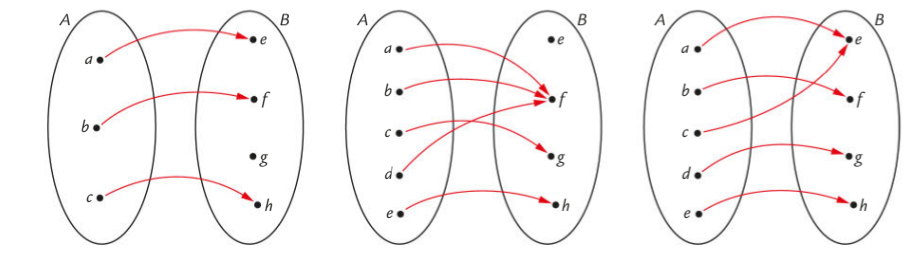
\includegraphics[width=\linewidth]{images/insiemi_funzioni.png}
\[ \text{a)} \hspace{60pt} \text{b)} \hspace{60pt} \text{c)} \]
\begin{solution}
Si applicano le definizioni leggendo le frecce del diagramma. Una funzione da $A$ a $B$ è:
\begin{itemize}
\item \textbf{iniettiva} se elementi distinti di $A$ hanno immagini distinte, cioè in ogni elemento di $B$ arriva \emph{al più} una freccia;
\item \textbf{suriettiva} se ogni elemento di $B$ è immagine di almeno un elemento di $A$, cioè in ogni elemento di $B$ arriva \emph{almeno} una freccia;
\item \textbf{biiettiva} se è insieme iniettiva e suriettiva, cioè in ogni elemento di $B$ arriva \emph{esattamente} una freccia.
\end{itemize}
Per ciascun diagramma a), b), c) si conta quante frecce arrivano su ogni elemento di $B$: nessun elemento con due frecce $\Rightarrow$ iniettiva; nessun elemento senza frecce $\Rightarrow$ suriettiva; entrambe le condizioni $\Rightarrow$ biiettiva.
\end{solution}
\end{question}

%----------------------------------------------------%

\begin{question}[ID=1.2, subtitle={Riconoscere funzioni da diagrammi a frecce}, difficulty=facile, tags={funzioni, insiemi}]
Stabilisci quali delle relazioni tra $A$ a $B$ rappresentate nei seguenti diagrammi a frecce sono funzioni.
\newline

\centering
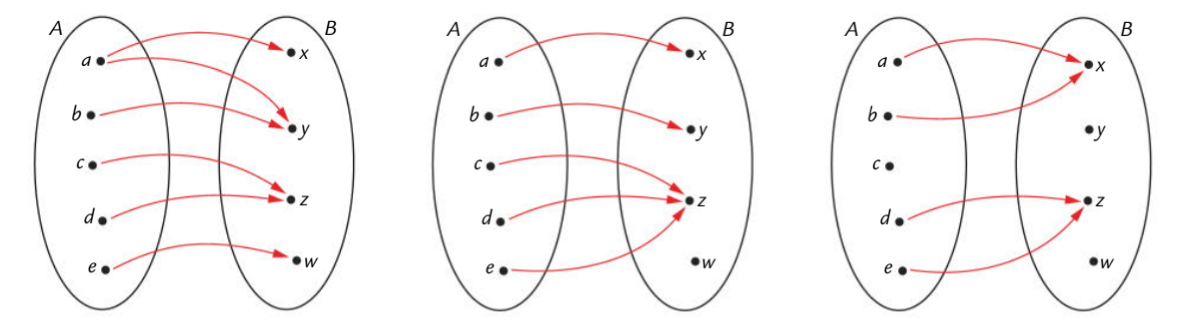
\includegraphics[width=0.9\linewidth]{images/insiemi_funzioni_1.png}
\[ \text{a)} \hspace{50pt} \text{b)} \hspace{50pt} \text{c)} \]
\begin{solution}
Una relazione da $A$ a $B$ è una \textbf{funzione} se a \emph{ogni} elemento di $A$ è associato \emph{uno e un solo} elemento di $B$. Quindi una relazione \emph{non} è funzione se da qualche elemento di $A$ parte più di una freccia (immagine non unica) oppure non parte alcuna freccia (immagine mancante). Per ciascun diagramma a), b), c) basta verificare che da ogni punto di $A$ esca esattamente una freccia: in tal caso è una funzione, altrimenti no.
\end{solution}
\end{question}




%====================================================%
% SEZIONE 2: Dominio
%====================================================%

\begin{question}[ID=2.1, subtitle={Dominio di funzioni razionali}, difficulty=facile, tags={dominio,razionali}]
Determinare il dominio delle seguenti funzioni:
\begin{center}\begin{minipage}{0.92\linewidth}
\begin{multicols}{2}
\begin{enumerate}[leftmargin=3.2cm]
\item $f(x)=\dfrac{2x+1}{x-3}$
\item $f(x)=\dfrac{x^2-4}{x^2-9}$
\item $f(x)=\dfrac{5}{x^3+1}$
\item $f(x)=\dfrac{x-2}{\sqrt{x^2-1}}$
\end{enumerate}
\end{multicols}
\end{minipage}\end{center}
\begin{solution}
Si escludono i valori che annullano i denominatori e si impone l'argomento delle radici di indice pari $\ge 0$ (e $>0$ se a denominatore). \\
a) Denominatore $x-3\neq0$: $D=\mathbb{R}\setminus\{3\}$. \\
b) $x^2-9\neq0\Rightarrow x\neq\pm3$: $D=\mathbb{R}\setminus\{-3,3\}$. \\
c) $x^3+1\neq0\Rightarrow x\neq-1$: $D=\mathbb{R}\setminus\{-1\}$. \\
d) La radice è a denominatore, quindi $x^2-1>0\Rightarrow x<-1$ o $x>1$: $D=(-\infty,-1)\cup(1,+\infty)$.
\end{solution}
\end{question}
%----------------------------------------------------%

%----------------------------------------------------%
\begin{question}[ID=2.2, subtitle={Dominio di funzioni irrazionali con radicali}, difficulty=facile, tags={dominio,radicali}]
Determinare il dominio delle seguenti funzioni:

\begin{center}\begin{minipage}{0.92\linewidth}
\begin{multicols}{2}
\begin{enumerate}[leftmargin=3.2cm]
\item $f(x)=\sqrt{4x-1}$
\item $f(x)=\sqrt{2-|x|}$
\item $f(x)=\dfrac{\sqrt{x+6}}{x-1}$
\item $f(x)=\sqrt[3]{\dfrac{x-2}{x+3}}$
\end{enumerate}
\end{multicols}
\end{minipage}\end{center}
\begin{solution}
a) Radice di indice pari: $4x-1\ge0\Rightarrow x\ge\dfrac14$: $D=\left[\dfrac14,+\infty\right)$. \\
b) $2-|x|\ge0\Rightarrow |x|\le2$: $D=[-2,2]$. \\
c) Numeratore: $x+6\ge0\Rightarrow x\ge-6$; denominatore: $x\neq1$: $D=[-6,1)\cup(1,+\infty)$. \\
d) La radice cubica esiste per ogni argomento reale; basta che la frazione sia definita, cioè $x+3\neq0$: $D=\mathbb{R}\setminus\{-3\}$.
\end{solution}
\end{question}

%----------------------------------------------------%

\begin{question}[ID=2.3, subtitle={Dominio con valore assoluto e composizioni}, difficulty=media, tags={dominio,assoluto,composizione}]
Determinare il dominio delle seguenti funzioni:

\begin{center}\begin{minipage}{0.92\linewidth}
\begin{multicols}{2}
\begin{enumerate}[leftmargin=3.2cm]
\item $f(x)=\sqrt{|x|-2}$
\item $f(x)=\dfrac{1}{|x-1|-2}$
\item $f(x)=\sqrt{(x-1)(5-x)}$
\item $f(x)=\dfrac{|x+2|}{\sqrt{x-3}}$
\end{enumerate}
\end{multicols}
\end{minipage}\end{center}
\begin{solution}
a) $|x|-2\ge0\Rightarrow |x|\ge2\Rightarrow x\le-2$ o $x\ge2$: $D=(-\infty,-2]\cup[2,+\infty)$. \\
b) $|x-1|-2\neq0\Rightarrow |x-1|\neq2\Rightarrow x\neq3$ e $x\neq-1$: $D=\mathbb{R}\setminus\{-1,3\}$. \\
c) Prodotto $\ge0$: $(x-1)(5-x)\ge0\Rightarrow 1\le x\le5$: $D=[1,5]$. \\
d) Radice a denominatore: $x-3>0\Rightarrow x>3$: $D=(3,+\infty)$.
\end{solution}
\end{question}
%----------------------------------------------------%

%----------------------------------------------------%
\begin{question}[ID=2.4, subtitle={Dominio di funzioni trigonometriche}, difficulty=media, tags={dominio,trigonometria}]
Determinare il dominio delle seguenti funzioni:

\begin{center}\begin{minipage}{0.92\linewidth}
\begin{multicols}{2}
\begin{enumerate}[leftmargin=3.2cm]
\item $f(x)=\dfrac{1}{\sin x}$
\item $f(x)=\tan(3x)$
\item $f(x)=\dfrac{1}{1-\cos(2x)}$
\item $f(x)=\sqrt{\sin x + 1}$
\end{enumerate}
\end{multicols}
\end{minipage}\end{center}
\begin{solution}
Con $k\in\mathbb{Z}$. \\
a) $\sin x\neq0\Rightarrow x\neq k\pi$: $D=\mathbb{R}\setminus\{k\pi\}$. \\
b) La tangente non esiste dove il suo argomento è $\dfrac{\pi}{2}+k\pi$: $3x\neq\dfrac{\pi}{2}+k\pi\Rightarrow x\neq\dfrac{\pi}{6}+\dfrac{k\pi}{3}$. \\
c) $1-\cos(2x)\neq0\Rightarrow\cos(2x)\neq1\Rightarrow 2x\neq2k\pi\Rightarrow x\neq k\pi$: $D=\mathbb{R}\setminus\{k\pi\}$. \\
d) $\sin x+1\ge0$ è sempre vero perché $\sin x\ge-1$: $D=\mathbb{R}$.
\end{solution}
\end{question}
%----------------------------------------------------%

%----------------------------------------------------%
\begin{question}[ID=2.5, subtitle={Dominio di funzioni composte con radicali annidati}, difficulty=difficile, tags={dominio,funzioni composte,radicali}]
Determinare il dominio delle seguenti funzioni:

\begin{center}\begin{minipage}{0.92\linewidth}
\begin{multicols}{2}
\begin{enumerate}[leftmargin=3.2cm]
\item $f(x)=\sqrt{\sqrt{x-1}-1}$
\item $f(x)=\dfrac{\sqrt{x-2}}{\sqrt{x-5}}$
\item $f(x)=\sqrt{\dfrac{x-4}{x-6}}$
\item $f(x)=\dfrac{\sqrt{|x+1|-1}}{x-2}$
\end{enumerate}
\end{multicols}
\end{minipage}\end{center}
\begin{solution}
a) Radice annidata: serve $x-1\ge0$ e $\sqrt{x-1}-1\ge0\Rightarrow\sqrt{x-1}\ge1\Rightarrow x-1\ge1\Rightarrow x\ge2$: $D=[2,+\infty)$. \\
b) Numeratore: $x-2\ge0$ ($x\ge2$); denominatore (radice, $>0$): $x-5>0$ ($x>5$). Intersezione: $D=(5,+\infty)$. \\
c) Frazione sotto radice $\ge0$: $\dfrac{x-4}{x-6}\ge0\Rightarrow x\le4$ o $x>6$ (escluso $x=6$): $D=(-\infty,4]\cup(6,+\infty)$. \\
d) $|x+1|-1\ge0\Rightarrow |x+1|\ge1\Rightarrow x\le-2$ o $x\ge0$; inoltre $x\neq2$: $D=(-\infty,-2]\cup[0,2)\cup(2,+\infty)$.
\end{solution}
\end{question}

%====================================================%
% SEZIONE 3: Funzioni iniettive, suriettive e biettive
%====================================================%


\begin{question}[ID=3.1, subtitle={Classificare funzioni da grafici — serie 1}, difficulty=facile, tags={funzioni,grafici}]
Osserva i seguenti grafici di funzioni e indica per ciascuno se la funzione è iniettiva, suriettiva, biettiva o nessuna delle tre opzioni.
\begin{center}
% Grafico 1
\begin{minipage}{0.24\textwidth}
\centering
\begin{tikzpicture}
\begin{axis}[
    axis y line=center, axis x line=middle,
    xmin=-2, xmax=8, ymin=-4, ymax=4,
    xlabel=$x$,ylabel=$y$, xtick=\empty, ytick=\empty,
    width=1.3\linewidth, height=1.3\linewidth
]
    \addplot [smooth, red, thick, mark=none, domain=-8:8,samples=200] {ln (x)};
\end{axis}
\end{tikzpicture}
\\ a)
\end{minipage}
% Grafico 2
\begin{minipage}{0.24\textwidth}
\centering
\begin{tikzpicture}
\begin{axis}[
    axis y line=center, axis x line=middle,
    xmin=-5, xmax=5, ymin=-10, ymax=10,
    xlabel=$x$,ylabel=$y$, xtick=\empty, ytick=\empty,
    width=1.3\linewidth, height=1.3\linewidth
]
    \addplot [smooth, red, thick, mark=none, domain=-5:5,samples=40] {x^3-4*x^2+5};
\end{axis}
\end{tikzpicture}
\\ b)
\end{minipage}
% Grafico 3
\begin{minipage}{0.24\textwidth}
\centering
\begin{tikzpicture}
\begin{axis}[
    axis y line=center, axis x line=middle,
    xmin=-3, xmax=3, ymin=-10, ymax=10,
    xlabel=$x$,ylabel=$y$, xtick=\empty, ytick=\empty,
    width=1.3\linewidth, height=1.3\linewidth
]
    \addplot [smooth, red, thick, mark=none, domain=-3:3,samples=40] {x^3};
\end{axis}
\end{tikzpicture}
\\ c)
\end{minipage}
% Grafico 4
\begin{minipage}{0.24\textwidth}
\centering
\begin{tikzpicture}
\begin{axis}[axis lines=middle, xlabel=$x$, ylabel=$y$, width=1.3\linewidth, height=1.3\linewidth,
xtick=\empty, ytick=\empty, xmin=-6.5, xmax=6.5, ymin=-1.5, ymax=1.5]
\addplot[domain=-6.28:6.28, samples=100, thick, red] {sin(deg(x))};
\end{axis}
\end{tikzpicture}
\\ d)
\end{minipage}
\end{center}
\begin{solution}
Si usa il criterio della retta orizzontale (iniettività: ogni retta $y=k$ taglia il grafico al più una volta) e si confronta l'insieme dei valori assunti con il codominio $\mathbb{R}$ (suriettività). \\
a) $y=\ln x$: strettamente crescente (iniettiva) e assume tutti i valori reali, quindi \textbf{biiettiva}. \\
b) $y=x^3-4x^2+5$: ha un massimo e un minimo relativi, quindi una retta orizzontale può tagliarla 3 volte (non iniettiva); essendo di grado dispari assume tutti i valori di $\mathbb{R}$ (suriettiva): \textbf{solo suriettiva}. \\
c) $y=x^3$: strettamente crescente e a valori in tutto $\mathbb{R}$: \textbf{biiettiva}. \\
d) $y=\sin x$: periodica (non iniettiva) e a valori in $[-1,1]\neq\mathbb{R}$ (non suriettiva): \textbf{nessuna delle tre}.
\end{solution}
\end{question}

%----------------------------------------------------%

\begin{question}[ID=3.2, subtitle={Classificare funzioni da grafici — serie 2}, difficulty=facile, tags={funzioni,grafici}]
Osserva i seguenti grafici di funzioni e indica per ciascuno se la funzione è iniettiva, suriettiva, biettiva o nessuna delle tre opzioni.
\begin{center}
% Grafico 1
\begin{minipage}{0.24\textwidth}
\centering
\begin{tikzpicture}
\begin{axis}[
    axis y line=center, axis x line=middle,
    xmin=-2, xmax=2, ymin=-4, ymax=4,
    xlabel=$x$,ylabel=$y$, xtick=\empty, ytick=\empty,
    width=1.3\linewidth, height=1.3\linewidth
]
    \addplot [smooth, red, thick, mark=none, domain=-8:8,samples=200] {x^2 -2};
\end{axis}
\end{tikzpicture}
\\ a)
\end{minipage}
% Grafico 2
\begin{minipage}{0.24\textwidth}
\centering
\begin{tikzpicture}
\begin{axis}[
    axis y line=center, axis x line=middle,
    xmin=-5, xmax=5, ymin=-10, ymax=10,
    xlabel=$x$,ylabel=$y$, xtick=\empty, ytick=\empty,
    width=1.3\linewidth, height=1.3\linewidth
]
    \addplot [smooth, red, thick, mark=none, domain=-5:5,samples=40] {x^3-4*x^2+5};
\end{axis}
\end{tikzpicture}
\\ b)
\end{minipage}
% Grafico 3
\begin{minipage}{0.24\textwidth}
\centering
\begin{tikzpicture}
\begin{axis}[
    axis y line=center, axis x line=middle,
    xmin=-3, xmax=3, ymin=-10, ymax=10,
    xlabel=$x$,ylabel=$y$, xtick=\empty, ytick=\empty,
    width=1.3\linewidth, height=1.3\linewidth
]
    \addplot [smooth, red, thick, mark=none, domain=0:3,samples=40] {2*x};
\end{axis}
\end{tikzpicture}
\\ c)
\end{minipage}
% Grafico 4
\begin{minipage}{0.24\textwidth}
\centering
\begin{tikzpicture}
\begin{axis}[axis lines=middle, xlabel=$x$, ylabel=$y$, width=1.3\linewidth, height=1.3\linewidth,
xtick=\empty, ytick=\empty, xmin=-4, xmax=4, ymin=-1.5, ymax=1.5]
\addplot[domain=-4:4, samples=100, thick, red] {x*e^x};
\end{axis}
\end{tikzpicture}
\\ d)
\end{minipage}
\end{center}
\begin{solution}
Come per la serie precedente, si valutano iniettività (retta orizzontale) e suriettività (valori assunti rispetto a $\mathbb{R}$). \\
a) $y=x^2-2$: parabola simmetrica rispetto all'asse $y$ (non iniettiva); valori in $[-2,+\infty)\neq\mathbb{R}$ (non suriettiva): \textbf{nessuna delle tre}. \\
b) $y=x^3-4x^2+5$: non iniettiva ma a valori in tutto $\mathbb{R}$: \textbf{solo suriettiva}. \\
c) $y=2x$ ristretta a $[0,3]$: retta crescente (iniettiva), ma i valori sono $[0,6]\neq\mathbb{R}$ (non suriettiva): \textbf{solo iniettiva}. \\
d) $y=x\,e^x$: ha un minimo in $x=-1$ (non iniettiva) e valori in $\left[-\tfrac{1}{e},+\infty\right)\neq\mathbb{R}$ (non suriettiva): \textbf{nessuna delle tre}.
\end{solution}
\end{question}

%====================================================%
% SEZIONE 4: Funzione inversa
%====================================================%

\begin{question}[ID=4.1, subtitle={Funzione inversa — serie 1}, difficulty=media, tags={funzioni,inversa}]
Determinare, se possibile, la funzione inversa delle seguenti funzioni:

\begin{center}\begin{minipage}{0.92\linewidth}
\begin{multicols}{2}
\begin{enumerate}[leftmargin=3.2cm]
\item $f(x)=2x+3$
\item $f(x)=\frac{x-1}{3}$
\item $f(x)=\frac{1}{x+2}$
\item $f(x)=\sqrt{x+5}$
\end{enumerate}
\end{multicols}
\end{minipage}\end{center}
\begin{solution}
Per invertire si scambiano $x$ e $y$ e si risolve rispetto a $y$. \\
a) $y=2x+3\Rightarrow f^{-1}(x)=\dfrac{x-3}{2}$. \\
b) $y=\dfrac{x-1}{3}\Rightarrow f^{-1}(x)=3x+1$. \\
c) $y=\dfrac{1}{x+2}\Rightarrow f^{-1}(x)=\dfrac{1}{x}-2=\dfrac{1-2x}{x}$, con $x\neq0$. \\
d) $y=\sqrt{x+5}$ (con $y\ge0$) $\Rightarrow f^{-1}(x)=x^2-5$, definita per $x\ge0$.
\end{solution}

\end{question}

%----------------------------------------------------%

\begin{question}[ID=4.2, subtitle={Funzione inversa — serie 2}, difficulty=media, tags={funzioni,inversa}]
Determinare, se possibile, la funzione inversa delle seguenti funzioni:

\begin{center}\begin{minipage}{0.92\linewidth}
\begin{multicols}{2}
\begin{enumerate}[leftmargin=3.2cm]
\item $f(x)=\frac{x+4}{5}$
\item $f(x)=3x-7$
\item $f(x)=\frac{2}{x-1}$
\item $f(x)=\sqrt{2x+3}$
\end{enumerate}
\end{multicols}
\end{minipage}\end{center}
\begin{solution}
Si scambiano $x$ e $y$ e si risolve per $y$. \\
a) $y=\dfrac{x+4}{5}\Rightarrow f^{-1}(x)=5x-4$. \\
b) $y=3x-7\Rightarrow f^{-1}(x)=\dfrac{x+7}{3}$. \\
c) $y=\dfrac{2}{x-1}\Rightarrow f^{-1}(x)=1+\dfrac{2}{x}=\dfrac{x+2}{x}$, con $x\neq0$. \\
d) $y=\sqrt{2x+3}\Rightarrow f^{-1}(x)=\dfrac{x^2-3}{2}$, definita per $x\ge0$.
\end{solution}

\end{question}

%----------------------------------------------------%

\begin{question}[ID=4.3, subtitle={Funzione inversa — serie 3}, difficulty=media, tags={funzioni,inversa}]
Determinare, se possibile, la funzione inversa delle seguenti funzioni:

\begin{center}\begin{minipage}{0.92\linewidth}
\begin{multicols}{2}
\begin{enumerate}[leftmargin=3.2cm]
\item $f(x)=5x-2$
\item $f(x)=\frac{x+3}{2}$
\item $f(x)=\frac{1}{x-4}$
\item $f(x)=\sqrt{x-1}$
\end{enumerate}
\end{multicols}
\end{minipage}\end{center}
\begin{solution}
a) $y=5x-2\Rightarrow f^{-1}(x)=\dfrac{x+2}{5}$. \\
b) $y=\dfrac{x+3}{2}\Rightarrow f^{-1}(x)=2x-3$. \\
c) $y=\dfrac{1}{x-4}\Rightarrow f^{-1}(x)=\dfrac{1}{x}+4=\dfrac{1+4x}{x}$, con $x\neq0$. \\
d) $y=\sqrt{x-1}\Rightarrow f^{-1}(x)=x^2+1$, definita per $x\ge0$.
\end{solution}

\end{question}

%----------------------------------------------------%

\begin{question}[ID=4.4, subtitle={Funzione inversa — serie 4}, difficulty=media, tags={funzioni,inversa}]
Determinare la funzione inversa delle seguenti funzioni:

\begin{center}\begin{minipage}{0.92\linewidth}
\begin{multicols}{2}
\begin{enumerate}[leftmargin=3.2cm]
\item $f(x)=\frac{2x-1}{3}$
\item $f(x)=4x+5$
\item $f(x)=\frac{3}{x+2}$
\item $f(x)=\sqrt{3x-4}$
\end{enumerate}
\end{multicols}
\end{minipage}\end{center}
\begin{solution}
a) $y=\dfrac{2x-1}{3}\Rightarrow f^{-1}(x)=\dfrac{3x+1}{2}$. \\
b) $y=4x+5\Rightarrow f^{-1}(x)=\dfrac{x-5}{4}$. \\
c) $y=\dfrac{3}{x+2}\Rightarrow f^{-1}(x)=\dfrac{3}{x}-2=\dfrac{3-2x}{x}$, con $x\neq0$. \\
d) $y=\sqrt{3x-4}\Rightarrow f^{-1}(x)=\dfrac{x^2+4}{3}$, definita per $x\ge0$.
\end{solution}

\end{question}

%----------------------------------------------------%

\begin{question}[ID=4.5, subtitle={Funzione inversa — serie 5}, difficulty=media, tags={funzioni,inversa}]
Determinare, se possibile, la funzione inversa delle seguenti funzioni:

\begin{center}\begin{minipage}{0.92\linewidth}
\begin{multicols}{2}
\begin{enumerate}[leftmargin=3.2cm]
\item $f(x)=7x+1$
\item $f(x)=\frac{x-5}{6}$
\item $f(x)=\frac{4}{x-3}$
\item $f(x)=\sqrt{5x+2}$
\end{enumerate}
\end{multicols}
\end{minipage}\end{center}
\begin{solution}
a) $y=7x+1\Rightarrow f^{-1}(x)=\dfrac{x-1}{7}$. \\
b) $y=\dfrac{x-5}{6}\Rightarrow f^{-1}(x)=6x+5$. \\
c) $y=\dfrac{4}{x-3}\Rightarrow f^{-1}(x)=\dfrac{4}{x}+3=\dfrac{4+3x}{x}$, con $x\neq0$. \\
d) $y=\sqrt{5x+2}\Rightarrow f^{-1}(x)=\dfrac{x^2-2}{5}$, definita per $x\ge0$.
\end{solution}

\end{question}

%====================================================%
% SEZIONE 5: Funzioni composte
%====================================================%

\begin{question}[ID=5.1, subtitle={Funzione composta $(f\circ g)(x)$ — serie 1}, difficulty=media, tags={funzioni,composte}]
Determinare la funzione composta \( (f\circ g)(x) \) per le seguenti coppie di funzioni:

\begin{center}\begin{minipage}{0.92\linewidth}
\begin{multicols}{2}
\begin{enumerate}[leftmargin=3.2cm]
\item $f(x)=2x+1, g(x)=x-3$
\item $f(x)=x^2, g(x)=x+2$
\item $f(x)=\sqrt{x}, g(x)=3x-1$
\item $f(x)=\frac{1}{x}, g(x)=x+4$
\end{enumerate}
\end{multicols}
\end{minipage}\end{center}
\begin{solution}
Per definizione $(f\circ g)(x)=f\big(g(x)\big)$: si sostituisce $g(x)$ al posto della variabile in $f$. \\
a) $f(g(x))=2(x-3)+1=2x-5$. \\
b) $f(g(x))=(x+2)^2$. \\
c) $f(g(x))=\sqrt{3x-1}$. \\
d) $f(g(x))=\dfrac{1}{x+4}$.
\end{solution}
\end{question}

%----------------------------------------------------%

\begin{question}[ID=5.2, subtitle={Funzione composta $(f\circ g)(x)$ — serie 2}, difficulty=media, tags={funzioni,composte}]
Determinare la funzione composta \( (f\circ g)(x) \) per le seguenti coppie di funzioni:

\begin{center}\begin{minipage}{0.92\linewidth}
\begin{multicols}{2}
\begin{enumerate}[leftmargin=3.2cm]
\item $f(x)=3x-2, g(x)=x^2$
\item $f(x)=\sqrt{x}, g(x)=2x+5$
\item $f(x)=\frac{1}{x}, g(x)=x-1$
\item $f(x)=x^2+1, g(x)=\sqrt{x}$
\end{enumerate}
\end{multicols}
\end{minipage}\end{center}
\begin{solution}
$(f\circ g)(x)=f\big(g(x)\big)$. \\
a) $f(g(x))=3x^2-2$. \\
b) $f(g(x))=\sqrt{2x+5}$. \\
c) $f(g(x))=\dfrac{1}{x-1}$. \\
d) $f(g(x))=(\sqrt{x})^2+1=x+1$, per $x\ge0$.
\end{solution}
\end{question}

%----------------------------------------------------%

\begin{question}[ID=5.3, subtitle={Funzione composta $(f\circ g)(x)$ — serie 3}, difficulty=media, tags={funzioni,composte}]
Determinare la funzione composta \( (f\circ g)(x) \) per le seguenti coppie di funzioni:

\begin{center}\begin{minipage}{0.92\linewidth}
\begin{multicols}{2}
\begin{enumerate}[leftmargin=3.2cm]
\item $f(x)=5x+3, g(x)=x-4$
\item $f(x)=x^2-1, g(x)=2x+1$
\item $f(x)=\sqrt{x+2}, g(x)=x^2$
\item $f(x)=\frac{1}{x-3}, g(x)=x+5$
\end{enumerate}
\end{multicols}
\end{minipage}\end{center}
\begin{solution}
$(f\circ g)(x)=f\big(g(x)\big)$. \\
a) $f(g(x))=5(x-4)+3=5x-17$. \\
b) $f(g(x))=(2x+1)^2-1=4x^2+4x$. \\
c) $f(g(x))=\sqrt{x^2+2}$. \\
d) $f(g(x))=\dfrac{1}{(x+5)-3}=\dfrac{1}{x+2}$.
\end{solution}
\end{question}

%----------------------------------------------------%

\begin{question}[ID=5.4, subtitle={Funzione composta $(f\circ g)(x)$ — serie 4}, difficulty=media, tags={funzioni,composte}]
Determinare la funzione composta \( (f\circ g)(x) \) per le seguenti coppie di funzioni:

\begin{center}\begin{minipage}{0.92\linewidth}
\begin{multicols}{2}
\begin{enumerate}[leftmargin=3.2cm]
\item $f(x)=2x^2, g(x)=x+1$
\item $f(x)=x+3, g(x)=\sqrt{x}$
\item $f(x)=\frac{1}{x+2}, g(x)=2x-1$
\item $f(x)=\sqrt{3x-5}, g(x)=x^2+1$
\end{enumerate}
\end{multicols}
\end{minipage}\end{center}
\begin{solution}
$(f\circ g)(x)=f\big(g(x)\big)$. \\
a) $f(g(x))=2(x+1)^2$. \\
b) $f(g(x))=\sqrt{x}+3$. \\
c) $f(g(x))=\dfrac{1}{(2x-1)+2}=\dfrac{1}{2x+1}$. \\
d) $f(g(x))=\sqrt{3(x^2+1)-5}=\sqrt{3x^2-2}$.
\end{solution}
\end{question}

%----------------------------------------------------%

\begin{question}[ID=5.5, subtitle={Funzione composta $(f\circ g)(x)$ — serie 5}, difficulty=media, tags={funzioni,composte}]
Determinare la funzione composta \( (f\circ g)(x) \) per le seguenti coppie di funzioni:

\begin{center}\begin{minipage}{0.92\linewidth}
\begin{multicols}{2}
\begin{enumerate}[leftmargin=3.2cm]
\item $f(x)=x^2+2, g(x)=x-3$
\item $f(x)=3x-4, g(x)=\sqrt{x}$
\item $f(x)=\frac{1}{x-1}, g(x)=x^2+1$
\item $f(x)=\sqrt{x+5}, g(x)=2x-3$
\end{enumerate}
\end{multicols}
\end{minipage}\end{center}
\begin{solution}
$(f\circ g)(x)=f\big(g(x)\big)$. \\
a) $f(g(x))=(x-3)^2+2$. \\
b) $f(g(x))=3\sqrt{x}-4$. \\
c) $f(g(x))=\dfrac{1}{(x^2+1)-1}=\dfrac{1}{x^2}$. \\
d) $f(g(x))=\sqrt{(2x-3)+5}=\sqrt{2x+2}$.
\end{solution}
\end{question}

%====================================================%
% SEZIONE 6: Miscellanea
%====================================================%

\begin{question}[ID=6.1, subtitle={Composizione e inverse di $f(x)=x-1$ e $g(x)=x^3$}, difficulty=difficile, tags={funzioni,composte,inversa}]
Date le funzioni
\[
f(x)=x-1,\quad g(x)=x^3,
\]
\begin{enumerate}
    \item Determinare \(f \circ g\) e \(g \circ f\);
    \item Giustificare perché le funzioni sono invertibili e determinare le espressioni di \(f^{-1}\) e \(g^{-1}\);
    \item Verificare che risulta $(f \circ g)^{-1} = g^{-1} \circ f^{-1}$
\end{enumerate}
\begin{solution}
\begin{enumerate}
\item $(f\circ g)(x)=f\big(g(x)\big)=x^3-1$;\quad $(g\circ f)(x)=g\big(f(x)\big)=(x-1)^3$.
\item $f(x)=x-1$ è una funzione lineare, quindi strettamente crescente e biiettiva: invertibile, con $f^{-1}(x)=x+1$. Anche $g(x)=x^3$ è strettamente crescente su tutto $\mathbb{R}$: invertibile, con $g^{-1}(x)=\sqrt[3]{x}$.
\item Da $(f\circ g)(x)=x^3-1$, ponendo $y=x^3-1$ si ricava $x=\sqrt[3]{y+1}$, quindi $(f\circ g)^{-1}(x)=\sqrt[3]{x+1}$. D'altra parte $(g^{-1}\circ f^{-1})(x)=g^{-1}\big(f^{-1}(x)\big)=g^{-1}(x+1)=\sqrt[3]{x+1}$. Le due espressioni coincidono, come previsto dalla regola dell'inversa di una composizione (l'ordine si scambia).
\end{enumerate}
\end{solution}
\end{question}

%----------------------------------------------------%

\begin{question}[ID=6.2, subtitle={Parametro $a$ per $g\circ f$ passante per $(0,4)$}, difficulty=difficile, tags={funzioni,composte,inversa}]
Date le funzioni $f(x)=3x^{2}-x$ e $g(x)=2x-a$, determina $a$ in modo che il grafico della funzione $g \circ f$ intersechi l'asse $y$ nel punto di coordinate $(0,4)$.
\begin{solution}
Calcoliamo la composizione: $(g\circ f)(x)=g\big(f(x)\big)=2(3x^2-x)-a=6x^2-2x-a$. L'intersezione con l'asse $y$ si ha in $x=0$, dove $(g\circ f)(0)=-a$. Imponendo il passaggio per $(0,4)$:
\[
-a=4 \;\Rightarrow\; \boxed{a=-4}.
\]
\end{solution}
\end{question}

%====================================================%
% FAC
%====================================================%
\begin{question}[ID=fac.1, subtitle={FAC: $f(f(f(x)))=8x+21$, trovare $a+b$}, headings=empty, difficulty=difficile, tags={funzioni,parametrico}]
\textbf{FAC)}
Supponi che \(f(x) = ax + b\), dove \(a\) e \(b\) sono numeri reali. Sapendo che \(f(f(f(x))) = 8x + 21\), quanto vale \(a + b\)?
\begin{solution}
Componendo tre volte una funzione lineare: $f(f(x))=a(ax+b)+b=a^2x+b(a+1)$ e quindi
\[
f(f(f(x)))=a^3x+b(a^2+a+1).
\]
Confrontando con $8x+21$: dal coefficiente di $x$, $a^3=8\Rightarrow a=2$; dal termine noto, $b(a^2+a+1)=7b=21\Rightarrow b=3$. Pertanto $a+b=\boxed{5}$.
\end{solution}
\end{question}

%----------------------------------------------------%

\begin{question}[ID=fac.2, subtitle={FAC: funzione con $f(x)+f(1/(1-x))=x$, trovare $f(2)$}, headings=empty, difficulty=difficile, tags={funzioni,parametrico}]
\textbf{FAC)}
Sia $f(x)$ una funzione tale che $f(x) + f\Big(\dfrac{1}{1-x}\Big) = x$ per tutte le $x$ diverse da 0 e da 1. Quanto vale $f(2)$?
\begin{solution}
La trasformazione $t(x)=\dfrac{1}{1-x}$ è ciclica di periodo 3: applicandola si ottiene $t(x)=\dfrac{1}{1-x}$, poi $t\big(t(x)\big)=\dfrac{x-1}{x}$, e infine $t\big(t(t(x))\big)=x$. Scrivendo l'equazione data per $x$, per $t(x)$ e per $t^2(x)$ otteniamo il sistema:
\[
f(x)+f\!\Big(\tfrac{1}{1-x}\Big)=x,\quad
f\!\Big(\tfrac{1}{1-x}\Big)+f\!\Big(\tfrac{x-1}{x}\Big)=\tfrac{1}{1-x},\quad
f\!\Big(\tfrac{x-1}{x}\Big)+f(x)=\tfrac{x-1}{x}.
\]
Sommando la prima e la terza e sottraendo la seconda si elimina tutto tranne $2f(x)$:
\[
f(x)=\tfrac12\Big(x+\tfrac{x-1}{x}-\tfrac{1}{1-x}\Big).
\]
Per $x=2$: $f(2)=\tfrac12\Big(2+\tfrac12-\tfrac{1}{-1}\Big)=\tfrac12\big(2+\tfrac12+1\big)=\boxed{\dfrac{7}{4}}$.
\end{solution}
\end{question}
